\documentclass[aspectratio=169,11pt]{beamer}
% Final report talk (30 min). Figures and numbers come from the final report sources.
\usepackage{amsmath,amssymb,bm}
\usepackage{graphicx}
\usepackage{booktabs}
\usepackage{multirow}
\usepackage{tikz}
\usetikzlibrary{positioning,arrows.meta,calc,fit,backgrounds,decorations.pathreplacing}
\usepackage{pgfplots}
\usepgfplotslibrary{groupplots,fillbetween}
\pgfplotsset{compat=1.18}
\usepackage{listings}

\definecolor{Navy}{HTML}{17365D}
\definecolor{Low}{HTML}{2F75B5}
\definecolor{High}{HTML}{D95545}
\definecolor{Ink}{HTML}{20252B}
\definecolor{Guide}{HTML}{D9DEE5}
\definecolor{Good}{HTML}{2E7D32}
\definecolor{CodeBg}{HTML}{F5F7FA}

\usefonttheme{professionalfonts}
\renewcommand{\familydefault}{\sfdefault}
\setlength{\parindent}{0pt}
\setbeamertemplate{navigation symbols}{}
\setbeamersize{text margin left=0.72cm,text margin right=0.72cm}
\setbeamercolor{normal text}{fg=Ink,bg=white}
\setbeamercolor{frametitle}{fg=Navy,bg=white}
\setbeamercolor{itemize item}{fg=Low}
\setbeamercolor{itemize subitem}{fg=Low}
\setbeamertemplate{itemize items}[circle]
\setbeamerfont{frametitle}{series=\bfseries,size=\fontsize{17.5}{20}}
\setbeamertemplate{frametitle}{%
  \vspace{0.22cm}\raggedright\insertframetitle\par
  \vspace{0.02cm}\textcolor{Guide}{\rule{\textwidth}{0.45pt}}}
\setbeamertemplate{footline}{%
  \leavevmode
  \begin{beamercolorbox}[wd=\paperwidth,ht=2.35ex,dp=1.0ex,leftskip=.3cm,rightskip=.30cm]{normal text}%
    {\fontsize{7}{8}\selectfont\color{gray}Collins--ISU WiCI \textbullet{} Final report: link-state forecasting}\hfill{\fontsize{7.5}{9}\selectfont\insertframenumber}
  \end{beamercolorbox}}
\newcommand{\takeaway}[1]{\vfill\centering{\fontsize{11.5}{14}\selectfont\color{Navy}\bfseries #1}\par}
\newcommand{\good}[1]{\textcolor{Good}{\textbf{#1}}}
\newcommand{\bad}[1]{\textcolor{High}{\textbf{#1}}}
\makeatletter\newcommand{\tabinput}[1]{\@@input #1 }\makeatother
\lstset{language=Python, basicstyle=\ttfamily\fontsize{7.3}{8.6}\selectfont, backgroundcolor=\color{CodeBg},
  keywordstyle=\color{Navy}\bfseries, commentstyle=\color{Good}\itshape, stringstyle=\color{High},
  frame=single, rulecolor=\color{Guide}, xleftmargin=2pt, xrightmargin=2pt, aboveskip=2pt, belowskip=2pt,
  showstringspaces=false, columns=fullflexible, keepspaces=true}

\input{data/plotstyle.tex}
\input{data/numbers_audit.tex}
\input{data/numbers_results.tex}
\input{data/numbers_analysis.tex}

\tikzset{s/.style={draw, rounded corners=3pt, align=center, text width=2.9cm, minimum height=2.1cm, fill=#1}}
\title{Final Report: Link-State Forecasting}
\author{Jalal Jalali, Evan Gossling, Daji Qiao, Hongwei Zhang}

\begin{document}

% 1 ------------------------------------------------------------------------
\begin{frame}[plain]
  \vspace{0.3cm}
  
\includegraphics[height=1.0cm]{collins_logo.jpeg}\hfill
\includegraphics[height=1.0cm]{wici_log3.png}\par
  \centering
  \vspace{0.7cm}
  {\fontsize{22}{26}\selectfont\color{Navy}\bfseries Integrated Terrestrial and Satellite Communications\par}
  \vspace{0.15cm}
  {\fontsize{14}{17}\selectfont\color{Low}\bfseries Final Report: Link-State Forecasting\\Audit, Distributional Models, and Calibrated Uncertainty\par}
  \vfill
  {\fontsize{10.5}{13}\selectfont Jalal Jalali \quad Evan Gossling \quad Daji Qiao \quad Hongwei Zhang\par}
  {\fontsize{8.7}{11}\selectfont Iowa State University \textbullet{} Center for Wireless, Communities and Innovation (WiCI)\par}
  \vspace{0.1cm}
  {\fontsize{8.7}{11}\selectfont Collins Aerospace: Naveen Rajanikantha, Ben Haan, Andrew Bys\par}
  \vspace{0.35cm}
\end{frame}

% 2 ------------------------------------------------------------------------
\begin{frame}{Outline}
  \begin{columns}[T,onlytextwidth]
  \begin{column}{0.5\textwidth}
  \begin{enumerate}
    \item Why forecast link state
    \item Where the earlier work left us
    \item Audit of the initial pipeline
    \item What we changed (4 steps, with code)
    \item How we evaluated
  \end{enumerate}
  \end{column}
  \begin{column}{0.5\textwidth}
  \begin{enumerate}\setcounter{enumi}{5}
    \item Results: accuracy and uncertainty
    \item Which change matters, and how sure we are
    \item Sensitivity studies
    \item What it means for the scheduler
    \item Limitations, next steps, deliverables
  \end{enumerate}
  \end{column}
  \end{columns}
  \vspace{0.6cm}
  \begin{block}{One-line summary}
  Against the initial model, on all six links: calibrated 95\% interval score \good{\ChgMISMean\%} and RTT MAE \good{\ChgMAEMean\%} on average, RMSE about unchanged.
  \end{block}
\end{frame}

% 3 ------------------------------------------------------------------------
\begin{frame}{Why forecast link state?}
  \begin{columns}[T,onlytextwidth]
  \begin{column}{0.52\textwidth}
  \begin{itemize}
    \item A terminal with \textbf{Starlink, OneWeb, and 5G} paths can send each packet on the best one.
    \item The earlier \textbf{liquid tunnel} (MPQUIC) does this, but schedulers react to \emph{past} RTT.
    \item LEO paths change fast:
    \begin{itemize}
      \item Starlink reallocates users every \textbf{15\,s}
      \item OneWeb RTT jumps at every handover
    \end{itemize}
    \item The earlier phase showed that forecasts help: prediction-aware minRTT cut frame loss per second by 52\%.
  \end{itemize}
  \end{column}
  \begin{column}{0.45\textwidth}
  \begin{block}{What the scheduler needs}
  \begin{itemize}
    \item RTT, jitter, loss forecasts\\ \textbf{0.2\,s to 3\,s} ahead, every 200\,ms
    \item \textbf{How wrong} each forecast may be\\ (a missed deadline is costly)
  \end{itemize}
  \end{block}
  \end{column}
  \end{columns}
  \takeaway{Point accuracy is not enough. The scheduler needs trustworthy uncertainty.}
\end{frame}

% 4 ------------------------------------------------------------------------
\begin{frame}{Where the earlier work left us}
  \begin{columns}[T,onlytextwidth]
  \begin{column}{0.5\textwidth}
  \begin{itemize}
    \item 8 models compared on 6 links\\(Starlink, OneWeb, 5G $\times$ DL/UL)
    \item \textbf{Seq2Seq-GRU} with attention selected as the primary model
    \item Targets: RTT, jitter, loss
    \item Input 30 rows, horizon 15 steps
    \item Reported PICP$_{95}\approx0.95$ everywhere\\``well-calibrated intervals''
  \end{itemize}
  \end{column}
  \begin{column}{0.48\textwidth}
  \textbf{Open questions for the final report}
  \begin{enumerate}
    \item Are the numbers right?\\(data pipeline, metrics)
    \item Can the forecasts be better?
    \item Can the uncertainty be trusted on sessions the model never saw?
  \end{enumerate}
  \end{column}
  \end{columns}
  \takeaway{Before improving the model, we rebuilt and audited the evaluation.}
\end{frame}

% 5 ------------------------------------------------------------------------
\begin{frame}{System model}
  \centering
  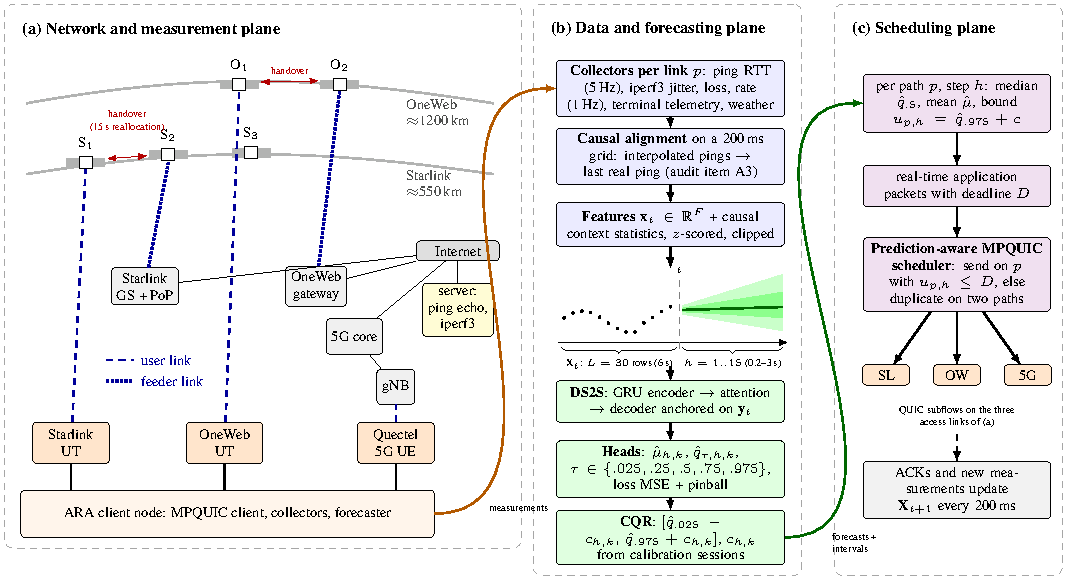
\includegraphics[height=0.8\textheight,width=\textwidth,keepaspectratio]{sysfig.pdf}
\end{frame}

% 6 ------------------------------------------------------------------------
\begin{frame}{Data: six links measured on the ARA living lab}
  \centering\small
  \begin{tabular}{lrrrrr}
  \toprule
  Link & Sessions (tr/va/te) & Train windows & Test windows & Features (Initial/Final) \\
  \midrule
  OneWeb DL   & 45 / 9 / 11   & 117{,}558 & 27{,}492  & 9 / 31 \\
  OneWeb UL   & 45 / 9 / 11   & 115{,}847 & 28{,}125  & 9 / 31 \\
  Starlink DL & 37 / 7 / 9    & 105{,}906 & 25{,}838  & 19 / 41 \\
  Starlink UL & 37 / 7 / 9    & 106{,}165 & 25{,}666  & 19 / 41 \\
  5G DL       & 266 / 57 / 58 & 194{,}725 & 169{,}204 & 10 / 32 \\
  5G UL       & 265 / 56 / 58 & 193{,}502 & 168{,}519 & 10 / 32 \\
  \bottomrule
  \end{tabular}
  \vspace{0.3cm}
  \begin{itemize}
    \item One row every \textbf{200\,ms}: input 30 rows = \textbf{6\,s}, horizon 15 steps = \textbf{0.2--3\,s}
    \item Split by \textbf{session} (70/15/15, seed 42), same as the earlier work: test sessions never seen
    \item 5G: every 4th training window used (7$\times$ more data), for all methods
  \end{itemize}
\end{frame}

% 7 ------------------------------------------------------------------------
\begin{frame}{Audit: six issues in the initial pipeline}
  \footnotesize
  \begin{tabular}{p{3.2cm}p{6.3cm}p{4.6cm}}
  \toprule
  Issue & Effect & Fix in the final report \\
  \midrule
  A1 Horizon unit & ``t+15s'' is really \textbf{3\,s} (200\,ms steps) & report $h\times0.2$\,s \\
  A2 Interval coverage & built from \textbf{test} residuals: 0.95 by construction & calibrate on validation sessions \\
  \textbf{A3 Starlink interpolation} & \bad{next ping leaks into the input} & last real ping, all methods \\
  A4 Constant targets & OneWeb UL jitter/loss always 0, $R^2=1$ in aggregate & per-target, $R^2$ undefined \\
  A5 ``Relative RMSE'' & not a persistence forecast & proper skill vs.\ $\hat y_{t+h}=y_t$ \\
  A6 One seed & report and stored run differ & 3 seeds + ensembles \\
  \bottomrule
  \end{tabular}
  \vspace{0.3cm}
  \begin{itemize}\small
    \item Reproduced the earlier results first: Starlink DL MAE \ReproSLMAE{} vs.\ 8.55, RMSE \ReproSLRMSE{} vs.\ 14.95
    \item 3 independent reviewers + 2 skeptics per finding, only surviving findings kept
  \end{itemize}
\end{frame}

% 8 ------------------------------------------------------------------------
\begin{frame}{A3: interpolation leaks the future into the input}
  \begin{columns}[T,onlytextwidth]
  \begin{column}{0.48\textwidth}
  \centering
  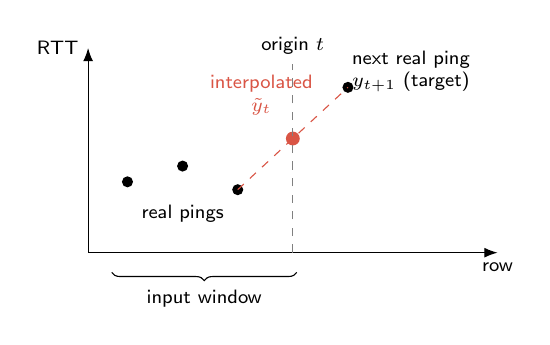
\begin{tikzpicture}[font=\scriptsize, >=Latex]
    \draw[->] (0,0) -- (5.2,0) node[below] {row};
    \draw[->] (0,0) -- (0,2.6) node[left] {RTT};
    \foreach \x/\y in {0.5/0.9, 1.2/1.1, 1.9/0.8} \fill (\x,\y) circle (2pt);
    \fill (3.3,2.1) circle (2pt);
    \draw[dashed, High] (1.9,0.8) -- (3.3,2.1);
    \fill[High] (2.6,1.45) circle (2.5pt);
    \draw[dashed, gray] (2.6,0) -- (2.6,2.4) node[above, black] {origin $t$};
    \node[High, align=center] at (2.2,2.0) {interpolated\\$\tilde y_t$};
    \node[align=center] at (4.1,2.3) {next real ping\\$y_{t+1}$ (target)};
    \node at (1.2,0.5) {real pings};
    \draw[decorate, decoration={brace, amplitude=3pt, mirror}] (0.3,-0.25) -- (2.65,-0.25) node[midway, below=3pt] {input window};
  \end{tikzpicture}
  \end{column}
  \begin{column}{0.5\textwidth}
  \textbf{Proposition (paper):} with $\tilde y_t=\tfrac12(y_{t-1}+y_{t+1})$,
  \[ y_{t+1}-\tilde y_t = \tfrac12\,(y_{t+1}-y_{t-1}) \]
  The persistence error is \textbf{halved}, and the squared error is \textbf{4$\times$ smaller}, on every interpolated row.
  \begin{itemize}\small
    \item \InterpFracSLDL\% of Starlink DL test targets interpolated
    \item fix raises 1-step persistence RMSE by \bad{\AuditPersHonePct\%}\\(\AuditPersLegacyHone{} $\rightarrow$ \AuditPersCausalHone\,ms)
    \item every interpolated origin lies strictly between its neighbors (100\%, vs.\ 47\% for real pings)
  \end{itemize}
  \end{column}
  \end{columns}
  \takeaway{All final results use causal inputs, for every method.}
\end{frame}

% 9 ------------------------------------------------------------------------
\begin{frame}[fragile]{The fix in code (\texttt{dataset.py})}
\begin{lstlisting}
def interpolated_mask(values):
    # Real pings have at most 3 decimals; time-interpolated values do not.
    v = pd.to_numeric(values, errors="coerce")
    return ((v * 1000 - (v * 1000).round()).abs() > 1e-3) & v.notna()

def causal_ping_fix(df, provider):
    """Keep the measured series as the TARGET, make the INPUT causal."""
    for col in INTERPOLATED_PING_COLS.get(provider, ()):
        v = pd.to_numeric(df[col], errors="coerce")
        m = interpolated_mask(v)
        df[col + "__orig"]   = v                    # used as target
        df[col + "__interp"] = m.astype("float32")  # for analysis
        df[col] = v.mask(m).ffill()                 # input = last real ping
\end{lstlisting}
  \vspace{0.2cm}
  \begin{itemize}\small
    \item Behind a flag: \texttt{DataConfig(causal\_ping=True)}, so the earlier results can still be reproduced exactly
    \item Applied to \textbf{every} method in the study, including the retrained initial model
  \end{itemize}
\end{frame}

% 10 -----------------------------------------------------------------------
\begin{frame}{What we changed: four steps}
  \centering
  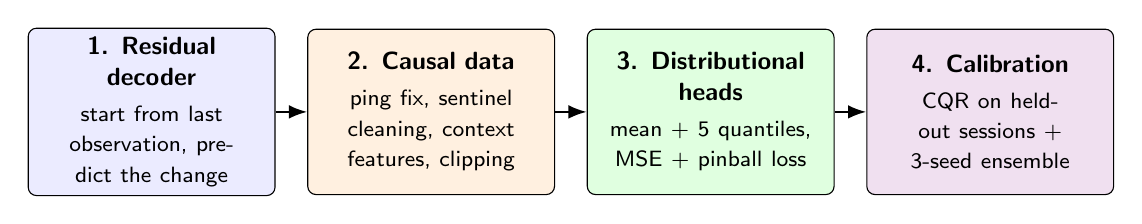
\begin{tikzpicture}[font=\small, >=Latex]
    \node[s=blue!8] (a) at (0,0) {\textbf{1. Residual}\\\textbf{decoder}\\[2pt]\footnotesize start from last observation, predict the change};
    \node[s=orange!12] (b) at (3.55,0) {\textbf{2. Causal data}\\[2pt]\footnotesize ping fix, sentinel cleaning, context features, clipping};
    \node[s=green!12] (c) at (7.1,0) {\textbf{3. Distributional}\\\textbf{heads}\\[2pt]\footnotesize mean + 5 quantiles, MSE + pinball loss};
    \node[s=violet!12] (d) at (10.65,0) {\textbf{4. Calibration}\\[2pt]\footnotesize CQR on held-out sessions + 3-seed ensemble};
    \draw[->, thick] (a) -- (b); \draw[->, thick] (b) -- (c); \draw[->, thick] (c) -- (d);
  \end{tikzpicture}
  \vspace{0.5cm}
  \begin{itemize}
    \item Encoder and attention are \textbf{unchanged} from the initial model, so the comparison isolates the decoder and the output
    \item Each step is evaluated separately (ablation, slide 23)
    \item New model: \texttt{models/seq2seq\_dist.py}, \ParamsDist{} parameters (initial model: \ParamsPrev)
  \end{itemize}
\end{frame}

% 11 -----------------------------------------------------------------------
\begin{frame}{Final forecaster}
  \centering
  \resizebox{0.78\textwidth}{!}{% final forecaster: GRU encoder, additive attention, residual autoregressive decoder.
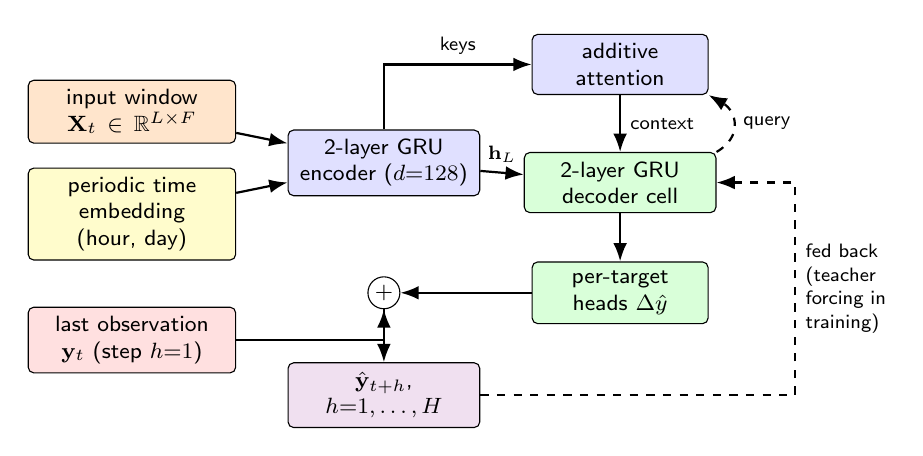
\begin{tikzpicture}[
  font=\footnotesize, >=Latex,
  b/.style={draw, rounded corners=2pt, minimum height=7mm, align=center, fill=#1},
  b/.default=gray!10,
  lnk/.style={->, thick}
]
\node[b=orange!20, text width=24mm] (in) at (0,0) {input window\\$\mathbf{X}_t\in\mathbb{R}^{L\times F}$};
\node[b=yellow!20, text width=24mm] (te) at (0,-1.3) {periodic time\\embedding (hour, day)};
\node[b=blue!12, text width=22mm] (enc) at (3.2,-0.65) {2-layer GRU\\encoder ($d{=}128$)};
\node[b=blue!12, text width=20mm] (att) at (6.2,0.6) {additive\\attention};
\node[b=green!15, text width=22mm] (dec) at (6.2,-0.9) {2-layer GRU\\decoder cell};
\node[b=green!15, text width=20mm] (head) at (6.2,-2.3) {per-target\\heads $\Delta\hat{y}$};
\node[draw, circle, inner sep=1pt, fill=white] (sum) at (3.2,-2.3) {$+$};
\node[b=red!12, text width=24mm] (last) at (0,-2.9) {last observation\\$\mathbf{y}_t$ (step $h{=}1$)};
\node[b=violet!12, text width=22mm] (out) at (3.2,-3.6) {$\hat{\mathbf{y}}_{t+h}$, $h{=}1,\dots,H$};
\draw[lnk] (in) -- (enc);
\draw[lnk] (te) -- (enc);
\draw[lnk] (enc) |- node[pos=0.75, above]{\scriptsize keys} (att);
\draw[lnk] (enc) -- node[above]{\scriptsize $\mathbf{h}_L$} (dec);
\draw[lnk] (att) -- node[right]{\scriptsize context} (dec);
\draw[lnk] (dec) -- (head);
\draw[lnk] (head) -- (sum);
\draw[lnk] (last) -| (sum);
\draw[lnk] (sum) -- (out);
\draw[lnk, dashed] (out.east) -| ++(4.0,0) |- node[pos=0.25, right, align=left]{\scriptsize fed back\\[-1pt]\scriptsize (teacher\\[-1pt]\scriptsize forcing in\\[-1pt]\scriptsize training)} (dec.east);
\draw[lnk, dashed] (dec.north east) to[out=30, in=-30, looseness=1.4] node[right]{\scriptsize query} (att.south east);
\end{tikzpicture}
}
  \takeaway{Persistence is the forecast when every head outputs zero. The network learns the departure from it.}
\end{frame}

% 12 -----------------------------------------------------------------------
\begin{frame}[fragile]{Steps 1--2: anchored decoder, context features}
  \begin{columns}[T,onlytextwidth]
  \begin{column}{0.52\textwidth}
\begin{lstlisting}
# decoder step (seq2seq_dist.py)
delta = torch.stack([head(top)
                     for head in self.heads], 1)
out   = last.unsqueeze(-1) + delta   # anchored
last  = out[..., 0]                  # feed back mean
\end{lstlisting}
  \vspace{0.1cm}
\begin{lstlisting}
# causal context features (dataset.py)
new[f"{c}__rsc"]    = rows_since_change(x)  # 0..10
new[f"{c}__mean5"]  = x.rolling(5).mean()    # 1 s
new[f"{c}__mean150"]= x.rolling(150).mean()  # 30 s
new[f"{c}__std300"] = x.rolling(300).std()   # 60 s
new[f"{c}__xmean"]  = x.expanding().mean()
\end{lstlisting}
  \end{column}
  \begin{column}{0.45\textwidth}
  \textbf{Why}
  \begin{itemize}\small
    \item The initial decoder started from \textbf{zero}, had to re-learn the level every time
    \item 6\,s window is short: rolling 30--60\,s statistics give longer context for free
    \item jitter/loss are 1\,Hz reports held 5 rows: ``rows since change'' gives the phase
    \item 5G logs contain SINR $=-32768$ sentinels: set to missing, clip $|z|\le5$
  \end{itemize}
  \end{column}
  \end{columns}
\end{frame}

% 13 -----------------------------------------------------------------------
\begin{frame}{Step 3: why a distribution instead of one number}
  \begin{columns}[T,onlytextwidth]
  \begin{column}{0.5\textwidth}
  \begin{itemize}
    \item RTT at 5\,Hz is \textbf{heavy tailed}: RMSE is \RatioRMSEMAEMin--\RatioRMSEMAEMax$\times$ the MAE\\(1.25$\times$ for Gaussian errors)
    \item A squared-error model learns the \textbf{mean}, which spikes pull upward
    \item Each loss has its own best forecast (Gneiting 2011):
    \begin{itemize}
      \item squared error $\rightarrow$ mean
      \item absolute error $\rightarrow$ median
      \item interval score $\rightarrow$ 2.5\% and 97.5\% quantiles
    \end{itemize}
  \end{itemize}
  \end{column}
  \begin{column}{0.47\textwidth}
  \begin{block}{Design}
  Each head outputs $\hat\mu$ and $\hat q_\tau$, $\tau\in\{.025,.25,.5,.75,.975\}$\\[4pt]
  Loss: $(\hat\mu-y)^2 + \tfrac15\sum_\tau \rho_\tau(y-\hat q_\tau)$\\[4pt]
  Report $\hat\mu$ for RMSE, $\hat q_{.5}$ for MAE, $[\hat q_{.025},\hat q_{.975}]$ for intervals
  \end{block}
  \end{column}
  \end{columns}
  \takeaway{One forward pass gives the right forecast for every use.}
\end{frame}

% 14 -----------------------------------------------------------------------
\begin{frame}[fragile]{Step 3 in code: quantile heads and loss}
\begin{lstlisting}
class DistHead(nn.Module):              # models/seq2seq_dist.py
    def forward(self, h):
        o = self.net(h)                  # 6 numbers per target and step
        mean, med = o[:, 0], o[:, 1]
        g = F.softplus(o[:, 2:]) + 1e-4  # positive gaps -> quantiles cannot cross
        q25, q75 = med - g[:, 0], med + g[:, 2]
        q025, q975 = q25 - g[:, 1], q75 + g[:, 3]
        return torch.stack([mean, q025, q25, med, q75, q975], dim=-1)

def dist_loss(out, y, quantile_weight=1.0):
    mse = ((out[..., 0] - y) ** 2).mean()                  # -> conditional mean
    tau = torch.tensor([0.025, 0.25, 0.5, 0.75, 0.975])
    e = y.unsqueeze(-1) - out[..., 1:]
    pinball = torch.maximum(tau * e, (tau - 1) * e).mean()  # -> conditional quantiles
    return mse + quantile_weight * pinball
\end{lstlisting}
  \small Extra cost: 4\% more parameters, \TimeDSCPU\,ms vs.\ \TimeSSCPU\,ms per forecast on one CPU thread (budget: 200\,ms).
\end{frame}

% 15 -----------------------------------------------------------------------
\begin{frame}[fragile]{Step 4: calibrate on unseen sessions}
  \begin{columns}[T,onlytextwidth]
  \begin{column}{0.5\textwidth}
  \textbf{Conformalized quantile regression (CQR)}
  \begin{itemize}\small
    \item score on validation windows:\\ $s_i=\max\{\hat q_{.025}-y_i,\ y_i-\hat q_{.975}\}$
    \item $c$ = the $\lceil(n{+}1)(0.95)\rceil$-th smallest score
    \item interval $[\hat q_{.025}-c,\ \hat q_{.975}+c]$, one $c$ per target and step
    \item Initial model: same, around its mean ($\hat y\pm c$)
    \item 3-seed ensemble: average mean and every quantile
  \end{itemize}
  \end{column}
  \begin{column}{0.48\textwidth}
\begin{lstlisting}
s = np.maximum(q_lo_val - y_val,
               y_val - q_hi_val)
k = np.ceil((n + 1) * (1 - alpha)) / n
c = np.quantile(s, k, method="higher")
lo, hi = q_lo_test - c, q_hi_test + c
\end{lstlisting}
  \small Deployment: offsets $c_{h,k}$ saved in\\ \texttt{summary/cqr\_offsets\_<link>.json}
  \end{column}
  \end{columns}
  \takeaway{Coverage is measured on test sessions, never computed from the test residuals.}
\end{frame}

% 16 -----------------------------------------------------------------------
\begin{frame}{How we evaluated}
  \begin{columns}[T,onlytextwidth]
  \begin{column}{0.5\textwidth}
  \textbf{Methods (same split, same causal data)}
  \begin{itemize}\small
    \item Persistence, 1\,s seasonal repeat
    \item Ridge and Ridge-E (tuned linear)
    \item \textbf{Initial} Seq2Seq-GRU, retrained
    \item Ablation: +residual, +data
    \item \textbf{Final} distributional + ensemble
  \end{itemize}
  \textbf{Protocol}
  \begin{itemize}\small
    \item 3 seeds per neural model, \NRuns{} runs + 80 sweep runs
    \item Original optimizer settings, early stopping (stopped after \EpochsMin--\EpochsMax{} epochs)
    \item Apple M3 Max GPU, about 7\,h
  \end{itemize}
  \end{column}
  \begin{column}{0.47\textwidth}
  \textbf{Metrics (test sessions)}
  \begin{itemize}\small
    \item MAE, RMSE, $R^2$ per target and step
    \item skill vs.\ persistence
    \item \textbf{interval score} (MIS):\\ width + $\tfrac2\alpha\times$ misses, lower is better
    \item coverage (PICP) of the calibrated 95\% interval
    \item per-session Wilcoxon test
  \end{itemize}
  \end{column}
  \end{columns}
\end{frame}

% 17 -----------------------------------------------------------------------
\begin{frame}{Headline: final vs.\ initial model on all six links (RTT)}
  \centering
  \begin{tikzpicture}
  \begin{axis}[ybar, width=0.95\textwidth, height=5.4cm, bar width=9pt, ymin=-45, ymax=5,
    symbolic x coords={OneWeb DL,OneWeb UL,Starlink DL,Starlink UL,5G DL,5G UL}, xtick=data,
    ylabel={change vs.\ the initial model (\%)}, legend style={at={(0.5,1.02)}, anchor=south, legend columns=3, font=\footnotesize},
    tick label style={font=\footnotesize}, ymajorgrids, grid style={gray!25}, nodes near coords, every node near coord/.append style={font=\tiny, anchor=north}]
  \addplot[fill=cFR] coordinates {(OneWeb DL,\ChgMISOWDL) (OneWeb UL,\ChgMISOWUL) (Starlink DL,\ChgMISSLDL) (Starlink UL,\ChgMISSLUL) (5G DL,\ChgMISQDL) (5G UL,\ChgMISQUL)};
  \addplot[fill=cRidge] coordinates {(OneWeb DL,\ChgMAEOWDL) (OneWeb UL,\ChgMAEOWUL) (Starlink DL,\ChgMAESLDL) (Starlink UL,\ChgMAESLUL) (5G DL,\ChgMAEQDL) (5G UL,\ChgMAEQUL)};
  \addplot[fill=cPers, nodes near coords={}] coordinates {(OneWeb DL,\ChgRMSEOWDL) (OneWeb UL,\ChgRMSEOWUL) (Starlink DL,\ChgRMSESLDL) (Starlink UL,\ChgRMSESLUL) (5G DL,\ChgRMSEQDL) (5G UL,\ChgRMSEQUL)};
  \legend{95\% interval score, MAE, RMSE}
  \end{axis}
  \end{tikzpicture}\par
  \small Seed means (3 seeds each). Coverage of the final model's 95\% intervals on test sessions: \PICPMin--\PICPMax.
  \takeaway{Interval score \ChgMISWorst\% to \ChgMISBest\%, MAE \ChgMAEWorst\% to \ChgMAEBest\%, RMSE about unchanged.}
\end{frame}

% 18 -----------------------------------------------------------------------
\begin{frame}{RTT results in detail: OneWeb and Starlink DL}
  \centering\small
  \resizebox{0.94\textwidth}{!}{%
  \begin{tabular}{llccccc}
  \toprule
  Link & Model & MAE (ms) & RMSE (ms) & $R^2$ & MIS (ms) & PICP \\
  \midrule
  \tabinput{data/tab_main_a.tex}
  \bottomrule
  \end{tabular}}
  \vfill\footnotesize Mean $\pm$ std over 3 seeds, and 3-seed ensembles. MIS: calibrated 95\% interval score. PICP: its measured coverage.
\end{frame}

\begin{frame}{RTT results in detail: Starlink UL and 5G}
  \centering\small
  \resizebox{0.94\textwidth}{!}{%
  \begin{tabular}{llccccc}
  \toprule
  Link & Model & MAE (ms) & RMSE (ms) & $R^2$ & MIS (ms) & PICP \\
  \midrule
  \tabinput{data/tab_main_b.tex}
  \bottomrule
  \end{tabular}}
  \vfill\footnotesize Mean $\pm$ std over 3 seeds, and 3-seed ensembles. MIS: calibrated 95\% interval score. PICP: its measured coverage.
\end{frame}

% 19 -----------------------------------------------------------------------
\begin{frame}{Per horizon step: RTT MAE}
  \centering
  \resizebox{!}{0.7\textheight}{\begin{tikzpicture}
\begin{groupplot}[group style={group size=3 by 2, horizontal sep=1.3cm, vertical sep=1.5cm}, frbase, width=5.3cm, height=4.0cm, xmin=0.2, xmax=3, xtick={0.2,1,2,3}, xlabel={horizon (s)}]
\nextgroupplot[title={OneWeb DL}, ylabel={RTT MAE (ms)}, legend to name=legMAE, legend columns=5]
\addplot[mRidge] table[x expr=\thisrow{h}*0.2, y=ridgefr] {data/h_oneweb_dl_rtt_MAE.dat};
\addlegendentry{Ridge-E}
\addplot[mPrev] table[x expr=\thisrow{h}*0.2, y=prevseq2seqens] {data/h_oneweb_dl_rtt_MAE.dat};
\addlegendentry{Initial Seq2Seq (3-seed ens.)}
\addplot[mResid] table[x expr=\thisrow{h}*0.2, y=frdist] {data/h_oneweb_dl_rtt_MAE.dat};
\addlegendentry{Final (seed mean)}
\addplot[mFR] table[x expr=\thisrow{h}*0.2, y=frdistens] {data/h_oneweb_dl_rtt_MAE.dat};
\addlegendentry{Final (3-seed ens.)}
\nextgroupplot[title={Starlink DL}]
\addplot[mRidge] table[x expr=\thisrow{h}*0.2, y=ridgefr] {data/h_starlink_dl_rtt_MAE.dat};
\addplot[mPrev] table[x expr=\thisrow{h}*0.2, y=prevseq2seqens] {data/h_starlink_dl_rtt_MAE.dat};
\addplot[mResid] table[x expr=\thisrow{h}*0.2, y=frdist] {data/h_starlink_dl_rtt_MAE.dat};
\addplot[mFR] table[x expr=\thisrow{h}*0.2, y=frdistens] {data/h_starlink_dl_rtt_MAE.dat};
\nextgroupplot[title={5G DL}]
\addplot[mRidge] table[x expr=\thisrow{h}*0.2, y=ridgefr] {data/h_quectel_dl_rtt_MAE.dat};
\addplot[mPrev] table[x expr=\thisrow{h}*0.2, y=prevseq2seqens] {data/h_quectel_dl_rtt_MAE.dat};
\addplot[mResid] table[x expr=\thisrow{h}*0.2, y=frdist] {data/h_quectel_dl_rtt_MAE.dat};
\addplot[mFR] table[x expr=\thisrow{h}*0.2, y=frdistens] {data/h_quectel_dl_rtt_MAE.dat};
\nextgroupplot[title={OneWeb UL}, ylabel={RTT MAE (ms)}]
\addplot[mRidge] table[x expr=\thisrow{h}*0.2, y=ridgefr] {data/h_oneweb_ul_rtt_MAE.dat};
\addplot[mPrev] table[x expr=\thisrow{h}*0.2, y=prevseq2seqens] {data/h_oneweb_ul_rtt_MAE.dat};
\addplot[mResid] table[x expr=\thisrow{h}*0.2, y=frdist] {data/h_oneweb_ul_rtt_MAE.dat};
\addplot[mFR] table[x expr=\thisrow{h}*0.2, y=frdistens] {data/h_oneweb_ul_rtt_MAE.dat};
\nextgroupplot[title={Starlink UL}]
\addplot[mRidge] table[x expr=\thisrow{h}*0.2, y=ridgefr] {data/h_starlink_ul_rtt_MAE.dat};
\addplot[mPrev] table[x expr=\thisrow{h}*0.2, y=prevseq2seqens] {data/h_starlink_ul_rtt_MAE.dat};
\addplot[mResid] table[x expr=\thisrow{h}*0.2, y=frdist] {data/h_starlink_ul_rtt_MAE.dat};
\addplot[mFR] table[x expr=\thisrow{h}*0.2, y=frdistens] {data/h_starlink_ul_rtt_MAE.dat};
\nextgroupplot[title={5G UL}]
\addplot[mRidge] table[x expr=\thisrow{h}*0.2, y=ridgefr] {data/h_quectel_ul_rtt_MAE.dat};
\addplot[mPrev] table[x expr=\thisrow{h}*0.2, y=prevseq2seqens] {data/h_quectel_ul_rtt_MAE.dat};
\addplot[mResid] table[x expr=\thisrow{h}*0.2, y=frdist] {data/h_quectel_ul_rtt_MAE.dat};
\addplot[mFR] table[x expr=\thisrow{h}*0.2, y=frdistens] {data/h_quectel_ul_rtt_MAE.dat};
\end{groupplot}
\node at ($(group c2r2.south)+(0,-1.25cm)$) {\pgfplotslegendfromname{legMAE}};
\end{tikzpicture}
}
  \takeaway{Final model below initial model at every step (0.2--3\,s) on every link.}
\end{frame}

\begin{frame}{Per horizon step: calibrated 95\% interval score}
  \centering
  \resizebox{!}{0.7\textheight}{\begin{tikzpicture}
\begin{groupplot}[group style={group size=3 by 2, horizontal sep=1.3cm, vertical sep=1.5cm}, frbase, width=5.3cm, height=4.0cm, xmin=0.2, xmax=3, xtick={0.2,1,2,3}, xlabel={horizon (s)}]
\nextgroupplot[title={OneWeb DL}, ylabel={RTT interval score (ms)}, legend to name=legMIS, legend columns=5]
\addplot[mRidge] table[x expr=\thisrow{h}*0.2, y=ridgefr] {data/h_oneweb_dl_rtt_MIS.dat};
\addlegendentry{Ridge-E}
\addplot[mPrev] table[x expr=\thisrow{h}*0.2, y=prevseq2seqens] {data/h_oneweb_dl_rtt_MIS.dat};
\addlegendentry{Initial Seq2Seq (3-seed ens.)}
\addplot[mResid] table[x expr=\thisrow{h}*0.2, y=frdist] {data/h_oneweb_dl_rtt_MIS.dat};
\addlegendentry{Final (seed mean)}
\addplot[mFR] table[x expr=\thisrow{h}*0.2, y=frdistens] {data/h_oneweb_dl_rtt_MIS.dat};
\addlegendentry{Final (3-seed ens.)}
\nextgroupplot[title={Starlink DL}]
\addplot[mRidge] table[x expr=\thisrow{h}*0.2, y=ridgefr] {data/h_starlink_dl_rtt_MIS.dat};
\addplot[mPrev] table[x expr=\thisrow{h}*0.2, y=prevseq2seqens] {data/h_starlink_dl_rtt_MIS.dat};
\addplot[mResid] table[x expr=\thisrow{h}*0.2, y=frdist] {data/h_starlink_dl_rtt_MIS.dat};
\addplot[mFR] table[x expr=\thisrow{h}*0.2, y=frdistens] {data/h_starlink_dl_rtt_MIS.dat};
\nextgroupplot[title={5G DL}]
\addplot[mRidge] table[x expr=\thisrow{h}*0.2, y=ridgefr] {data/h_quectel_dl_rtt_MIS.dat};
\addplot[mPrev] table[x expr=\thisrow{h}*0.2, y=prevseq2seqens] {data/h_quectel_dl_rtt_MIS.dat};
\addplot[mResid] table[x expr=\thisrow{h}*0.2, y=frdist] {data/h_quectel_dl_rtt_MIS.dat};
\addplot[mFR] table[x expr=\thisrow{h}*0.2, y=frdistens] {data/h_quectel_dl_rtt_MIS.dat};
\nextgroupplot[title={OneWeb UL}, ylabel={RTT interval score (ms)}]
\addplot[mRidge] table[x expr=\thisrow{h}*0.2, y=ridgefr] {data/h_oneweb_ul_rtt_MIS.dat};
\addplot[mPrev] table[x expr=\thisrow{h}*0.2, y=prevseq2seqens] {data/h_oneweb_ul_rtt_MIS.dat};
\addplot[mResid] table[x expr=\thisrow{h}*0.2, y=frdist] {data/h_oneweb_ul_rtt_MIS.dat};
\addplot[mFR] table[x expr=\thisrow{h}*0.2, y=frdistens] {data/h_oneweb_ul_rtt_MIS.dat};
\nextgroupplot[title={Starlink UL}]
\addplot[mRidge] table[x expr=\thisrow{h}*0.2, y=ridgefr] {data/h_starlink_ul_rtt_MIS.dat};
\addplot[mPrev] table[x expr=\thisrow{h}*0.2, y=prevseq2seqens] {data/h_starlink_ul_rtt_MIS.dat};
\addplot[mResid] table[x expr=\thisrow{h}*0.2, y=frdist] {data/h_starlink_ul_rtt_MIS.dat};
\addplot[mFR] table[x expr=\thisrow{h}*0.2, y=frdistens] {data/h_starlink_ul_rtt_MIS.dat};
\nextgroupplot[title={5G UL}]
\addplot[mRidge] table[x expr=\thisrow{h}*0.2, y=ridgefr] {data/h_quectel_ul_rtt_MIS.dat};
\addplot[mPrev] table[x expr=\thisrow{h}*0.2, y=prevseq2seqens] {data/h_quectel_ul_rtt_MIS.dat};
\addplot[mResid] table[x expr=\thisrow{h}*0.2, y=frdist] {data/h_quectel_ul_rtt_MIS.dat};
\addplot[mFR] table[x expr=\thisrow{h}*0.2, y=frdistens] {data/h_quectel_ul_rtt_MIS.dat};
\end{groupplot}
\node at ($(group c2r2.south)+(0,-1.25cm)$) {\pgfplotslegendfromname{legMIS}};
\end{tikzpicture}
}
  \takeaway{Largest gains on Starlink DL, OneWeb, and 5G UL, where RTT is bursty.}
\end{frame}

% 20 -----------------------------------------------------------------------
\begin{frame}{Why the intervals are better: they follow the input}
  \centering
  \resizebox{0.88\textwidth}{!}{\begin{tikzpicture}
\begin{axis}[frbase, width=0.95\linewidth, height=5.2cm, xlabel={time in test session (s)}, ylabel={Starlink DL RTT (ms)}, xmin=0, xmax=59.8, legend style={at={(0.5,1.03)}, anchor=south, legend columns=4}]
\addplot[name path=hi, draw=none, forget plot] table[x=t, y=frhi] {data/trace_starlink_dl.dat};
\addplot[name path=lo, draw=none, forget plot] table[x=t, y=frlo] {data/trace_starlink_dl.dat};
\addplot[cFR!25] fill between[of=hi and lo];
\addlegendentry{Final 95\% interval (CQR)}
\addplot[black, thin] table[x=t, y=truth] {data/trace_starlink_dl.dat};
\addlegendentry{measured}
\addplot[mPrev, mark=none] table[x=t, y=y2] {data/trace_starlink_dl.dat};
\addlegendentry{Initial (ens.)}
\addplot[cFR, thick] table[x=t, y=frmed] {data/trace_starlink_dl.dat};
\addlegendentry{Final median (ens.)}
\end{axis}
\end{tikzpicture}
}
  \begin{itemize}\small
    \item Final interval widens around bursts, narrows when calm. Width--error rank correlation \RhoMin--\RhoMax{} on all links
    \item Starlink DL 95\% interval: \textbf{100\,ms} wide (Final) vs.\ \textbf{176\,ms} (Initial), same coverage
  \end{itemize}
\end{frame}

% 21 -----------------------------------------------------------------------
\begin{frame}{Which step helps? (ablation vs.\ initial model)}
  \centering\tiny
  \setlength{\tabcolsep}{2.4pt}
  \begin{tabular}{l*{18}{r}}
  \toprule
  & \multicolumn{3}{c}{OneWeb DL} & \multicolumn{3}{c}{OneWeb UL} & \multicolumn{3}{c}{Starlink DL} & \multicolumn{3}{c}{Starlink UL} & \multicolumn{3}{c}{5G DL} & \multicolumn{3}{c}{5G UL} \\
  Steps & MAE & RMSE & MIS & MAE & RMSE & MIS & MAE & RMSE & MIS & MAE & RMSE & MIS & MAE & RMSE & MIS & MAE & RMSE & MIS \\
  \midrule
  \tabinput{data/tab_ablation.tex}
  \bottomrule
  \end{tabular}
  \vspace{0.4cm}
  \begin{itemize}\small
    \item Steps 1--2 alone do \textbf{not} lower the MAE (OneWeb DL $+9.8\%$, $+19\%$): a squared-error model anchored on a spiky value follows the spikes
    \item Step 2 helps the \textbf{mean}: up to $-4.5\%$ RMSE (Starlink DL)
    \item \good{The gains come from Step 3}, the distributional output. Ensembling adds up to 6 points
  \end{itemize}
\end{frame}

% 22 -----------------------------------------------------------------------
\begin{frame}{The evaluation method hides or shows the gain}
  \begin{columns}[T,onlytextwidth]
  \begin{column}{0.55\textwidth}
  \centering
  \resizebox{\linewidth}{!}{%
  \begin{tabular}{lrrrrrr}
  \toprule
  & \multicolumn{3}{c}{Earlier method} & \multicolumn{3}{c}{Calibrated} \\
  Link & Initial & Final & $\Delta$\% & Initial & Final & $\Delta$\% \\
  \midrule
  \tabinput{data/tab_isproto.tex}
  \bottomrule
  \end{tabular}}
  \end{column}
  \begin{column}{0.42\textwidth}
  \small
  RTT interval score (ms)
  \begin{itemize}
    \item \textbf{Earlier method}: quantiles of test residuals around the mean $\rightarrow$ both models within $\pm2\%$
    \item \textbf{Calibrated} on held-out sessions $\rightarrow$ final model 8--39\% better
  \end{itemize}
  \end{column}
  \end{columns}
  \takeaway{Test-residual intervals hide the value of input-dependent uncertainty and overstate coverage.}
\end{frame}

% 23 -----------------------------------------------------------------------
\begin{frame}{How sure are we? Per-session significance}
  \begin{columns}[T,onlytextwidth]
  \begin{column}{0.5\textwidth}
  \centering
  \resizebox{\linewidth}{!}{%
  \begin{tabular}{lrrrr}
  \toprule
  Link & Sessions & Final wins & Median $\Delta$\% & $p$ \\
  \midrule
  \tabinput{data/tab2_sessions.tex}
  \bottomrule
  \end{tabular}}
  \end{column}
  \begin{column}{0.46\textwidth}
  \begin{itemize}\small
    \item Windows of one session are correlated, so the \textbf{session} is the unit of evidence
    \item The final model has lower RTT MAE in \good{\SessWinsTotal{} of \SessNTotal} test sessions
    \item Wilcoxon $p<0.01$ on 5 of 6 links
    \item OneWeb UL: 8 of 11, not significant ($p=\SessPOWUL$)
  \end{itemize}
  \end{column}
  \end{columns}
\end{frame}

% 24 -----------------------------------------------------------------------
\begin{frame}{Honest comparison with simple baselines}
  \centering\scriptsize
  \setlength{\tabcolsep}{3pt}
  \begin{tabular}{l*{12}{r}}
  \toprule
  & \multicolumn{2}{c}{OneWeb DL} & \multicolumn{2}{c}{OneWeb UL} & \multicolumn{2}{c}{Starlink DL} & \multicolumn{2}{c}{Starlink UL} & \multicolumn{2}{c}{5G DL} & \multicolumn{2}{c}{5G UL} \\
  Method & MAE & skill & MAE & skill & MAE & skill & MAE & skill & MAE & skill & MAE & skill \\
  \midrule
  \tabinput{data/tab_baselines.tex}
  \bottomrule
  \end{tabular}
  \vspace{0.3cm}
  \begin{itemize}\small
    \item Persistence is poor at 5\,Hz (single pings are noisy). Starlink DL has a 1\,s pattern (seasonal repeat: 28\% skill)
    \item A tuned linear model (Ridge-E) is \textbf{within 1 point} of the initial network's RMSE skill on 4 links
    \item Final ensemble: \good{lowest MAE and highest skill on every link} (tied on 5G UL)
  \end{itemize}
\end{frame}

% 25 -----------------------------------------------------------------------
\begin{frame}{Sensitivity studies (80 extra runs, satellite links)}
  \centering\tiny
  \setlength{\tabcolsep}{3pt}
  \begin{tabular}{l*{12}{r}}
  \toprule
  & \multicolumn{3}{c}{OneWeb DL} & \multicolumn{3}{c}{OneWeb UL} & \multicolumn{3}{c}{Starlink DL} & \multicolumn{3}{c}{Starlink UL} \\
  Setting (Final vs.\ Initial, \%) & MAE & RMSE & MIS & MAE & RMSE & MIS & MAE & RMSE & MIS & MAE & RMSE & MIS \\
  \midrule
  \tabinput{data/tab3_sweeps_vs.tex}
  \bottomrule
  \end{tabular}
  \vspace{0.3cm}
  \begin{itemize}\small
    \item The final model beats the initial one in \textbf{every} window and horizon setting: MIS 7--41\% better, MAE lower everywhere
    \item \good{Pinball weight 4} (instead of 1) improves the final model further: OneWeb DL MAE $-10.4\%$. Our main tables understate the model
    \item Best window depends on the link (12\,s: OneWeb UL $-9.4\%$, OneWeb DL $+11.2\%$). Hidden size 128 is adequate
  \end{itemize}
\end{frame}

% 26 -----------------------------------------------------------------------
\begin{frame}{What it means for the multipath scheduler}
  \begin{columns}[T,onlytextwidth]
  \begin{column}{0.5\textwidth}
  \textbf{Per-path risk bound}
  \begin{itemize}\small
    \item $u_{p,h}=\hat q_{.975}+c$ holds $\approx$95\% of the time on unseen sessions
    \item send on path $p$ if $u_{p,h}\le$ deadline, else duplicate on two paths
    \item tight on calm paths $\Rightarrow$ fewer needless duplicates
  \end{itemize}
  \textbf{Spike warning} (RTT $>$ 90th pct., AUROC)
  \begin{itemize}\small
    \item Starlink DL: \good{\AUCFRSLDL} (Final) vs.\ \AUCPrevSLDL{} (Initial)
    \item similar on 4 links, worse on OneWeb DL\\(\AUCFROWDL{} vs.\ \AUCPrevOWDL)
  \end{itemize}
  \end{column}
  \begin{column}{0.47\textwidth}
  \textbf{Which output for which decision}
  \begin{itemize}\small
    \item \textbf{median} $\hat q_{.5}$: rank paths by expected delay
    \item \textbf{mean} $\hat\mu$: capacity, throughput estimates
    \item \textbf{upper bound}: deadline and duplication decisions
  \end{itemize}
  \vspace{0.2cm}
  \textbf{Real-time}: \TimeDSCPU\,ms per forecast on one CPU thread, every 200\,ms
  \end{column}
  \end{columns}
\end{frame}

% 27 -----------------------------------------------------------------------
\begin{frame}{Limitations and next steps}
  \begin{columns}[T,onlytextwidth]
  \begin{column}{0.5\textwidth}
  \textbf{Limitations}
  \begin{itemize}\small
    \item RTT \textbf{RMSE did not improve} by more than 7\% anywhere
    \item Coverage measured, not guaranteed (sessions not exchangeable)
    \item One site, constant-rate iperf traffic, one split
    \item iperf reports stamped at interval start
    \item Scheduler benefit argued, not yet measured end to end
  \end{itemize}
  \end{column}
  \begin{column}{0.47\textwidth}
  \textbf{Next steps}
  \begin{itemize}\small
    \item Run the final model inside the liquid tunnel (end-to-end video test)
    \item Pinball weight 4, per-link input window
    \item Cross-path features (state of the other links)
    \item Online (adaptive) conformal updates
    \item Fix iperf timestamps in the parsers
  \end{itemize}
  \end{column}
  \end{columns}
\end{frame}

% 28 -----------------------------------------------------------------------
\begin{frame}{Summary and deliverables}
  \begin{itemize}
    \item \textbf{Audit}: found and fixed a future-data leak in Starlink RTT and a coverage metric that was 0.95 by construction
    \item \textbf{Model}: same encoder, anchored decoder, \textbf{distributional heads}, CQR calibration, ensembles
    \item \textbf{Results}: interval score \good{8--39\%} better, MAE \good{2--18\%} lower, all six links, significant in 5 of 6
  \end{itemize}
  \vspace{0.2cm}
  \begin{block}{Deliverables (github.com/Jalalij/Collins\_2026)}
  \small
  final report (53 pages) \textbullet{} IEEE TWC paper draft (10 pages, 40 refs) \textbullet{} code and benchmark scripts \textbullet{} 202 trained models \textbullet{} measurement data \textbullet{} supplementary docs (changes, data audit, reproduction)
  \end{block}
  \takeaway{Questions?}
\end{frame}

\end{document}
